\chapter{Results}\label{chp:results}

All the mapping was done in the same machine equipped with an Intel Core i5-4430@3.00 GHz and 8 GB DDR3 memory. All the CPU measurements reflect the usage of a single core, meaning that values higher than 100\% represent the usage of more than one core at a time. The memory measurements are USS or "Unique Set Size", which is the amount of memory that would be freed if the process was terminated. The Gmapping version used was 1.3.10 \cite{gmappinggit}, the Hector version used was 0.3.5 \cite{hectorgit}, the Karto version used was 0.7.3 \cite{kartogit} and the Cartographer version used was 0.3.0 \cite{cartographergit}.

The mapping results for the three test maps selected on \prettyref{sec:selecting_maps} can be seen on \prettyref{fig:results1}, for the test map 1, \prettyref{fig:results2}, for the test map 2 and \prettyref{fig:results3} for the test map 3. The respective data collected during execution can be seen on \prettyref{tab:results1}, \prettyref{tab:results2} and \prettyref{tab:results3}.

At visual inspection, we can see that for the first map (\prettyref{fig:results1}), Karto Slam and Cartographer perform better, as the noise in the walls is lower. They look straight and sharp, as opposed to Gmapping and Hector, where the walls look noisy. If we inspect the results of \prettyref{tab:results1}, we can see that this reflects in Karto having the lowest localization error between all algorithms for this map for all metrics. Even though the Hector reconstruction is not as great, it scores second place in localization error, followed by Cartographer and finally Gmapping, although Cartographer is better at poses and Gmapping is better at angles.

In the second map, the results are quite the opposite, with Hector and Cartographer performing better visually. Hector shows the best pose estimate in disparity, but Gmapping wins in squared error. Karto remains with good results but Cartographer lags behind. We can actually see why looking at the map, as Cartographer's map is tilted relative to the others. This error of orientation at the start was probably what made Cartographer go perform in the localization.

In terms of average CPU and Memory usage, the values remained constant throughout the tests. Gmapping shows the highest usage of CPU among all algorithms, consuming almost double of Cartographer, in second place. Karto and Hector show low consumption of CPU, with Hector being the lowest. In terms of memory, Hector jumps ahead in all tests, followed by Gmapping, Hector and finally Cartographer. It is important to notice that despite having low CPU and memory footprint, we are only taking into consideration the SLAM node for Cartographer, and not the obstacle grid node nor the offline tasks executed by the \texttt{.pbstream} conversion.

\newpage
\begin{figure}[!ht]
     \centering
     \subfloat[][Gmapping]{\includegraphics[width=.4\linewidth]{gmapping/test1}\label{subfig:gmapping_test1}}
     \hspace{1cm}
     \subfloat[][Hector]{\includegraphics[width=.4\linewidth]{hector/test1}\label{subfig:hector_test1}}
     \\
     \subfloat[][Karto]{\includegraphics[width=.4\linewidth]{karto/test1}\label{subfig:karto_test1}}
     \hspace{1cm}
     \subfloat[][Cartographer]{\includegraphics[width=.4\linewidth]{cartographer/test1}\label{subfig:cartographer_test1}}
     \caption{Results of mapping for first map.}
     \label{fig:results1}
\end{figure}

\begin{table}[!ht]
\centering
\renewcommand*{\arraystretch}{1.1}
\begin{tabular}{c|c|c|c|c}
& \textbf{Gmapping} & \textbf{Hector} & \textbf{Karto} & \textbf{Cartographer} \\ \hline
\textbf{Pose disparity} & 0.0010116 & 0.00051379 & 0.00014934 & 0.00095104 \\
\textbf{Angle disparity} & 4.0385e-05 & 2.3272e-05 & 1.2402e-05 & 0.00010114 \\
\textbf{Pose squared error} & 0.0018224 & 0.00058361 & 0.00024294 & 0.00086193 \\
\textbf{Angle squared error} & 2.0899e-05 & 1.6251e-05 & 6.9566e-06 & 6.3385e-05 \\
\textbf{CPU (\%)} & 14.36 & 3.67 & 4.74 & 7.13 \\
\textbf{Memory (MB)} & 19.56 & 26.39 & 13.18 & 12.52 \\ \hline
\end{tabular}
\caption{Data collected for the first map (lower is better).}
\label{tab:results1}
\end{table}


\begin{figure}[!ht]
     \centering
     \subfloat[][Gmapping]{\includegraphics[width=.4\linewidth]{gmapping/test2}\label{subfig:gmapping_test2}}
     \hspace{1cm}
     \subfloat[][Hector]{\includegraphics[width=.4\linewidth]{hector/test2}\label{subfig:hector_test2}}
     \\
     \subfloat[][Karto]{\includegraphics[width=.4\linewidth]{karto/test2}\label{subfig:karto_test2}}
     \hspace{1cm}
     \subfloat[][Cartographer]{\includegraphics[width=.4\linewidth]{cartographer/test2}\label{subfig:cartographer_test2}}
     \caption{Results of mapping for second map.}
     \label{fig:results2}
\end{figure}

\begin{table}[!ht]
\centering
\renewcommand*{\arraystretch}{1.1}
\begin{tabular}{c|c|c|c|c}
& \textbf{Gmapping} & \textbf{Hector} & \textbf{Karto} & \textbf{Cartographer} \\ \hline
\textbf{Pose disparity} & 0.00037009 & 0.00024439 & 0.0031410 & 0.013768 \\
\textbf{Angle disparity} & 3.6161e-05 & 2.6309e-05 & 1.0607e-05 & 4.4936e-05 \\
\textbf{Pose squared error} & 0.00038672 & 0.0010135 & 0.0035834 & 0.013529 \\
\textbf{Angle squared error} & 0.00038672 & 2.5932e-05 & 0.00016662 & 0.00060306 \\
\textbf{CPU (\%)} & 11.38 & 3.75 & 4.72 & 6.56 \\
\textbf{Memory (MB)} & 19.11 & 26.50 & 14.45 & 12.33 \\ \hline
\end{tabular}
\caption{Data collected for the second map (lower is better).}
\label{tab:results2}
\end{table}

\begin{figure}[!ht]
     \centering
     \subfloat[][Gmapping]{\includegraphics[width=.4\linewidth]{gmapping/test3}\label{subfig:gmapping_test3}}
     \hspace{1cm}
     \subfloat[][Hector]{\includegraphics[width=.4\linewidth]{hector/test3}\label{subfig:hector_test3}}
     \\
     \subfloat[][Karto]{\includegraphics[width=.4\linewidth]{karto/test3}\label{subfig:karto_test3}}
     \hspace{1cm}
     \subfloat[][Cartographer]{\includegraphics[width=.4\linewidth]{cartographer/test3}\label{subfig:cartographer_test3}}
     \caption{Results of mapping for third map.}
     \label{fig:results3}
\end{figure}

\begin{table}[!ht]
\centering
\renewcommand*{\arraystretch}{1.1}
\begin{tabular}{c|c|c|c|c}
& \textbf{Gmapping} & \textbf{Hector} & \textbf{Karto} & \textbf{Cartographer} \\ \hline
\textbf{Pose disparity} & 0.015545 & 0.013457 & 0.0050207 & 0.0012753 \\
\textbf{Angle disparity} & 6.0892e-05 & 9.0999e-05 & 5.0616e-05 & 4.7758e-05 \\
\textbf{Pose squared error} & 0.022001 & 0.015299 & 0.0054754 & 0.0026521 \\
\textbf{Angle squared error} & 0.00055478 & 0.00080006 & 0.00033509 & 2.8089e-05 \\
\textbf{CPU (\%)} & 12.04 & 3.73 & 4.99 & 6.30 \\
\textbf{Memory (MB)} & 19.88 & 26.32 & 15.88 & 14.45 \\ \hline
\end{tabular}
\caption{Data collected for the third map (lower is better).}
\label{tab:results3}
\end{table}
\clearpage

In the third map, Cartographer seems to outperform every other algorithm in every metric, resulting in a much better map, followed by Karto, and finally Gmapping and Hector with very similar results. It is clear from analyzing the pose error from all the algorithm runs that this method is not giving a good way of measuring accuracy, at least for this test case.

The results of running the ICP matcher with the algorithms can be seen on \prettyref{tab:results_icp}. The best algorithm in all cases was Cartographer, scoring lowest. This means two things: most of the walls were placed in the correct spot and the noise is low. In the second place, Gmapping could outperform Hector and Karto, justifying the wide adoption of Gmapping in the robotic world, as it is far easier to set up than Cartographer. Hector and Karto were tied in the last position in this test, as Hector was better at the first map, Karto was better in the second map and the results are approximately the same in the third map.

\begin{table}[!ht]
\centering
\renewcommand*{\arraystretch}{1.1}
\begin{tabular}{c|c|c|c|c}
& \textbf{Gmapping} & \textbf{Hector} & \textbf{Karto} & \textbf{Cartographer} \\ \hline
\textbf{Test 1} & 0.46144 & 0.61088 & 0.75229 & 0.34752 \\
\textbf{Test 2} & 0.55829 & 0.76593 & 0.62868 & 0.51959 \\
\textbf{Test 3} & 0.64751 & 0.78693 & 0.75315 & 0.41721 \\
 \hline
\end{tabular}
\caption{Results of running ICP over maps (lower is better).}
\label{tab:results_icp}
\end{table}

When modeling free space, most of the algorithms show the same result, with Gmapping showing slightly better results than the other. One of the problems Gmapping faces, though, is mapping places inside the walls where it has no information about, as shown on \prettyref{fig:gmapping_error}. This results in more free space being shown than normal, which might indicate why Gmapping has a lower score. All the algorithms have results with a positive sign, meaning that the less free space was mapped than in fact exists, which is good, as discussed in \prettyref{sec:free_space}.

\begin{figure}[!ht]
     \centering
     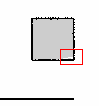
\includegraphics[width=.4\linewidth]{gmapping_error}
     \caption{Incorrect mapping from Gmapping on test 2.}
     \label{fig:gmapping_error}
\end{figure}

\begin{table}[!ht]
\centering
\renewcommand*{\arraystretch}{1.1}
\begin{tabular}{c|c|c|c|c}
& \textbf{Gmapping} & \textbf{Hector} & \textbf{Karto} & \textbf{Cartographer} \\ \hline
\textbf{Test 1 (\%)} & 3.71 & 4.15 & 4.98 & 4.91 \\
\textbf{Test 2 (\%)} & 3.68 & 4.80 & 4.61 & 6.09 \\
\textbf{Test 3 (\%)} & 3.90 & 5.24 & 5.02 & 5.79 \\
 \hline
\end{tabular}
\caption{Results of free space mapping accuracy (lower is better).}
\label{tab:results_whitespace}
\end{table}

We are going to analyze the CPU and Memory profiles for each algorithm running in the second map. Figures \ref{fig:gmapping_cpu} to \ref{fig:cartographer_cpu} show both the CPU usage and RAM Memory used over time. The $x$ axis represents the number of samples, and since the acquisition frequency was 10 Hz, every 500 samples are equivalent to 50 seconds.

\prettyref{fig:gmapping_cpu} shows how Gmapping performs when running. It is possible to see that the CPU peaks at a value of more than 100\% every few iterations, and most of the time it stays around 10\%. This peak every few iterations is the result of each laser scan being processed, and the effort seems to stay constant until the end, peaking around the same value. The memory grows in small incremental steps as the map is being constructed, and stops at around 1000 samples, where the map is already near the final state and only a few bits of new information are added.

\begin{figure}[!ht]
    \centering
    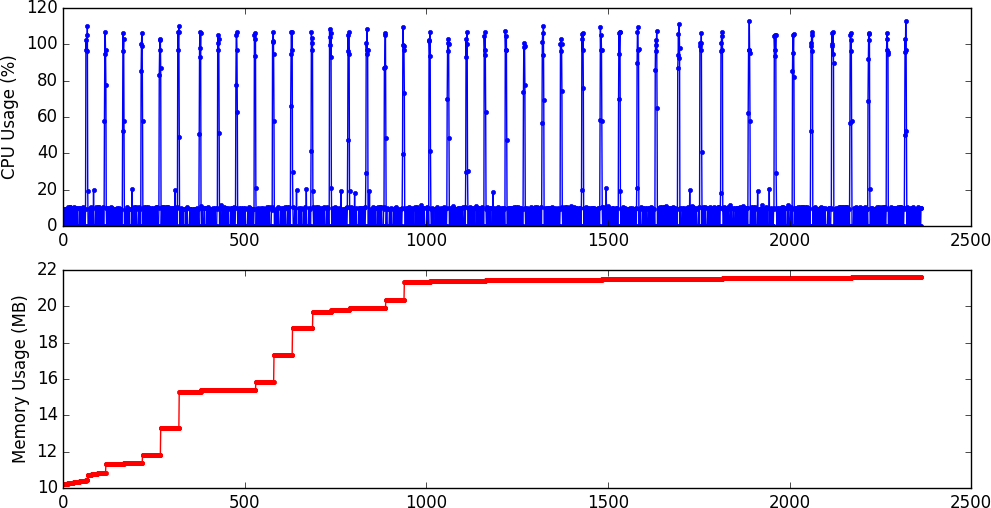
\includegraphics[width=.8\linewidth]{gmapping_cpu}
    \caption{CPU and Memory usage for Gmapping running map test 2.}
    \label{fig:gmapping_cpu}
\end{figure}

As already mentioned, Hector performs better on CPU and worse on memory. \prettyref{fig:hector_cpu} shows peaks around 20 \% and around 10 \%. Most of the time, the algorithm stays idle, to account for the average CPU usage of around 4 \%. Memory consumption, in this case, is high from the start and stays the same until the end. One of the reasons might be because it allocates the whole map right from the start, instead of allocating memory for a small map and increasing as new areas are discovered.

\begin{figure}[!ht]
    \centering
    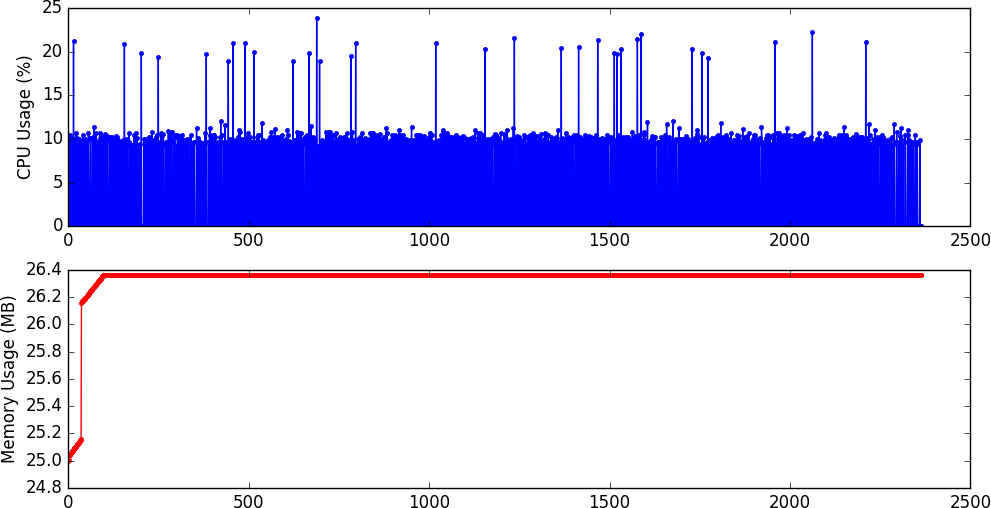
\includegraphics[width=.8\linewidth]{hector_cpu}
    \caption{CPU and Memory usage for Hector running map test 2.}
    \label{fig:hector_cpu}
\end{figure}

The results for Karto can be seen on \prettyref{fig:karto_cpu}. For CPU, we can see that the peaks become higher as the algorithm is executed for longer. This is expected as the problem of optimizing a pose-graph becomes harder as more nodes are added to the graph. The memory seems to grow linearly as time progresses, even though no more information is being added after some point in time.

\begin{figure}[!ht]
    \centering
    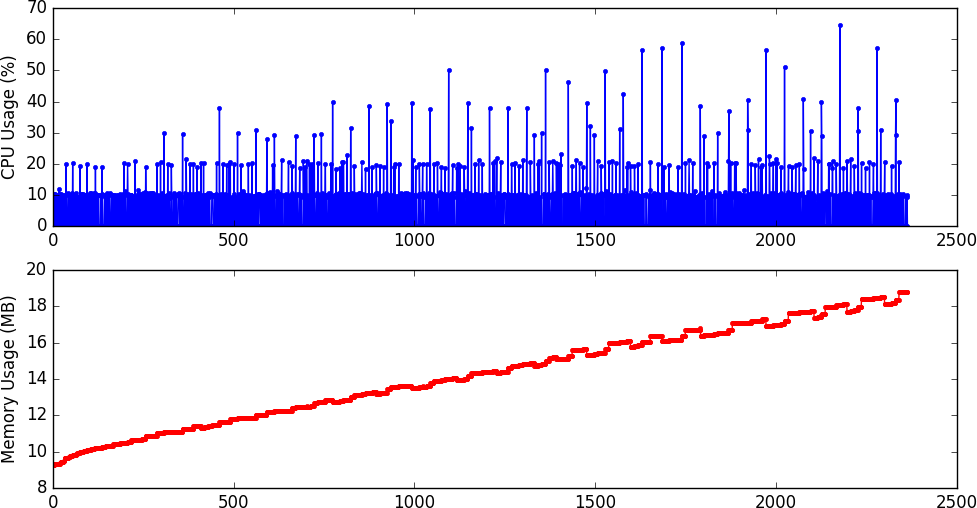
\includegraphics[width=.8\linewidth]{karto_cpu}
    \caption{CPU and Memory usage for Karto running map test 2.}
    \label{fig:karto_cpu}
\end{figure}

Finally, the results for Cartographer can be seen on \prettyref{fig:cartographer_cpu}. It behaves similar to Gmapping, although with lower peaks, with the memory growing linearly like Karto, with small bumps every 1000 samples.

\begin{figure}[!ht]
    \centering
    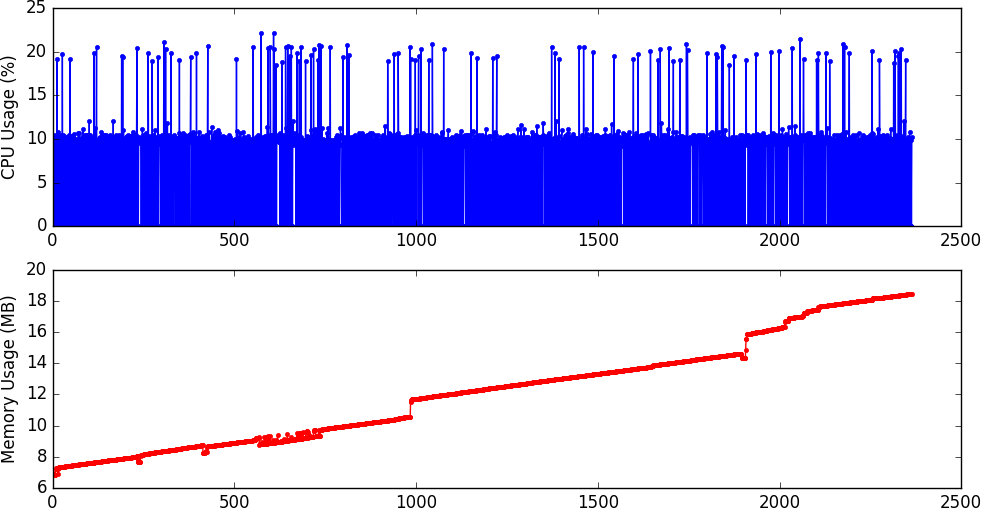
\includegraphics[width=.8\linewidth]{cartographer_cpu}
    \caption{CPU and Memory usage for Cartographer running map test 2.}
    \label{fig:cartographer_cpu}
\end{figure}

In terms of results, the temporal analysis of the graphs brings additional information to the table. All the algorithms show consumption around 10\%, differentiating on the peaks and the amount they stay idle. Gmapping was the most intensive on CPU, especially because of all the peaks. Hector and Karto stayed with low consumption and Cartographer were very modest considering its complexity. 